\documentclass[a4paper, 12pt]{article}
\usepackage[top=1.5cm, bottom=1.5cm, left=1.5cm, right=1.5cm]{geometry}
\usepackage{float}
\usepackage[utf8]{inputenc}
\usepackage{array}
\usepackage{geometry}
\usepackage{placeins}
\usepackage{pgfplots}
\pgfplotsset{compat=1.18}

\begin{document}
	\begin{center}
		Universidade Federal do Rio Grande do Norte
		
		Departamento de Engenharia da Computação e Automação  
		
		DCA3703 - Programação Paralela  
		
		\textbf{Tarefa 13: Afinidade de threads}  
		
		\textbf{Aluno:} Daniel Bruno Trindade da Silva  
	\end{center}  
	
	\section{Introdução}
	
	\hspace{0.62cm}Este relatório tem como objetivo apresentar os conhecimentos adquiridos durante a realização da Tarefa 13 da disciplina de \textbf{Computação Paralela}. A atividade consistiu em avaliar a escalabilidade do programa desenvolvido na Tarefa 11 — um simulador da velocidade de um fluido utilizando a equação de Navier-Stokes — aplicando diferentes políticas de afinidade de \textit{threads}.
	
	\section{Enunciado}
	
	\hspace{0.62cm}Avalie como a escalabilidade do seu código de Navier-Stokes muda ao utilizar os diversos tipos de afinidades de \textit{threads} suportados pelo sistema operacional e pelo OpenMP, no mesmo nó de computação do NPAD utilizado para a Tarefa 12.
	
	\section{Desenvolvimento}
	
	\hspace{0.62cm}Na Tarefa 11, desenvolvemos duas versões de um programa para simular a velocidade de um fluido: uma versão sequencial (serial) e outra paralelizada com OpenMP. Para a análise requerida nesta tarefa, utilizamos a versão paralelizada do código.
	
	Nesta tarefa, analisamos os impactos da cláusula \texttt{proc\_bind()} com as seguintes políticas de afinidade:
	
	\begin{itemize}
		\item \textbf{\texttt{spread}} — O openMP distribui as \textit{threads} de forma espalhada pelos processadores, maximizando a distância entre elas. O objetivo é utilizar o máximo de recursos do hardware possível, como diferentes \textit{sockets} ou núcleos físicos. Aumenta a latência de comunicação entre as \textit{threads} em troca de menos disputa por recurso. Ideal quando temos programas com \textit{threads} independentes;
		
		\item \textbf{\texttt{close}} — O openMP agrupa as \textit{threads} próximas umas das outras, preferencialmente no mesmo \textit{socket} ou núcleos adjacentes ao da \textit{thread} master. Utilizada quando queremos manter as \textit{threads} próximas pra diminuir a latência, mas não queremos sobrecarregar um mesmo núcleo;
		
		\item \textbf{\texttt{master}} — Nessa política todas as \textit{threads} são alocadas no mesmo local onde a \textit{thread} principal (\textit{master/primary}) está executando. Utilizado quando a comunicação entre \textit{threads} é muito intensa e isso compença a perda de paralelismo. Pois ela gera disputa por recursos, mas reduz a latência de comunicação entre as \textit{threads};
		
		\item \textbf{\texttt{true}} — herda a política de afinidade da região paralela pai. Se não houver região pai, comporta-se de acordo com a política padrão definida pela implementação.
		
		\item \textbf{\texttt{false}} — Desativa a afinidade de \textit{threads} o escalonador do sistema operacional é quem vai decidir onde cada \textit{thread} ficará. Com isso pode haver migração de \textit{threads} entre núcleos causando mais overhead e menos previsibilidade;
	\end{itemize}
	
	Reorganizamos o código de forma a possibilitar o teste de todas as políticas em uma única execução. Assim como realizado na Tarefa 12, o código foi executado com 1, 2, 4, 8, 16 e 32 \textit{threads}, para que ao final pudéssemos analisar se houve influência dessas políticas de afinidade na eficiência do código.
	
	O código foi executado no super computador da universidade utilizando o nó com o processador intel-128, cada teste foi executado 6 vezes para termos a certeza da constância dos resultados.
	
	\section{Resultados}
	\hspace{0.62cm}Iniciaremos avaliando a escalabilidade forte fixando o tamanho de nosso problema e aumentando o número de threads utilizados para o processamento. A figura abaixo mostra nossos resultados: 
	
	\begin{center}
		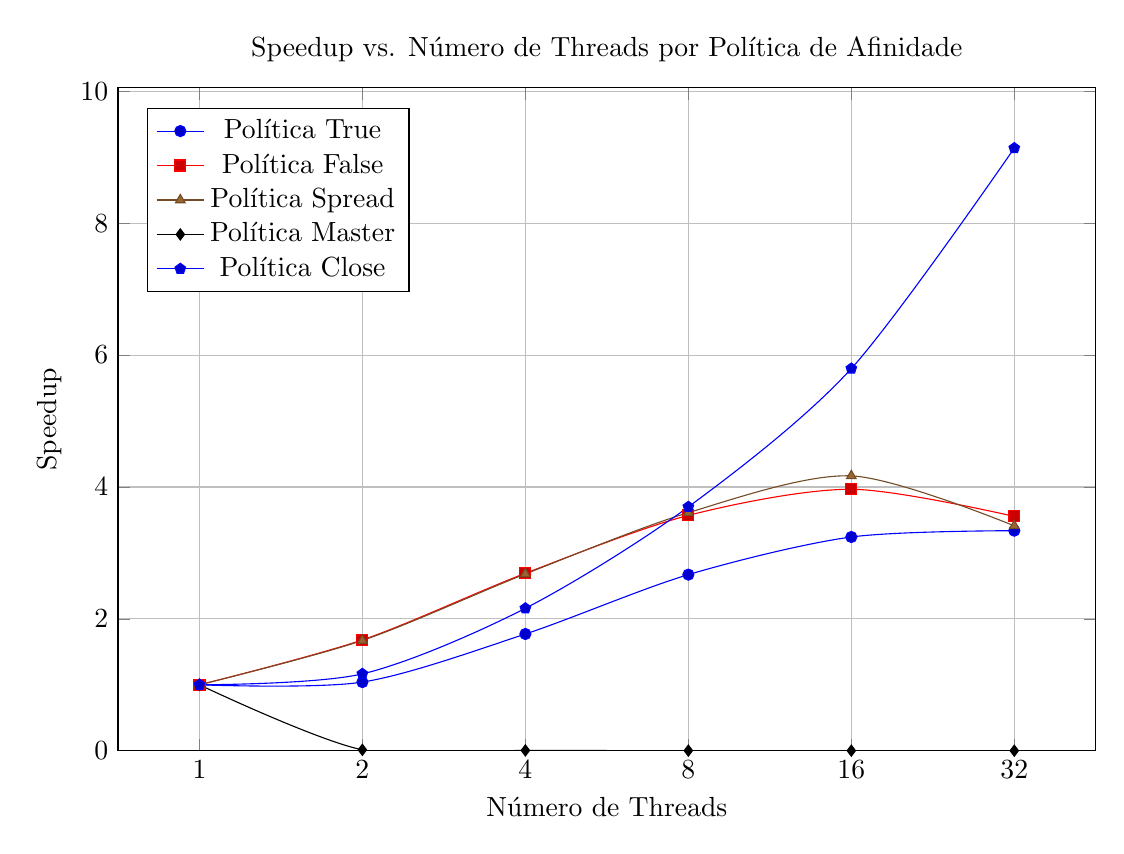
\begin{tikzpicture}
			\begin{axis}[
				title={Speedup vs. Número de Threads por Política de Afinidade},
				xlabel={Número de Threads},
				ylabel={Speedup},
				xmode=log,                      % Eixo X em escala logarítmica
				log ticks with fixed point,     % Formato dos ticks no eixo log
				xtick={1,2,4,8,16,32},
				xticklabels={1,2,4,8,16,32},
				legend pos=north west,          % Posição da legenda
				grid=major,                     % Adiciona grade principal
				width=14cm,                     % Largura do gráfico
				height=10cm,                    % Altura do gráfico
				ymin=0,                         % Valor mínimo do eixo Y
				% ymax pode ser ajustado conforme necessário, mas pgfplots geralmente lida bem automaticamente
				]
				
				% Dados para o gráfico
				% Politica True
				\addplot+[mark=*, smooth] coordinates {
					(1, 1.000000) (2, 1.041223) (4, 1.770291) (8, 2.670522) (16, 3.241188) (32, 3.337166)
				};
				\addlegendentry{Política True}
				
				% Politica False
				\addplot+[mark=square*, smooth] coordinates {
					(1, 1.000000) (2, 1.681153) (4, 2.691582) (8, 3.568715) (16, 3.965107) (32, 3.553509)
				};
				\addlegendentry{Política False}
				
				% Politica Spread
				\addplot+[mark=triangle*, smooth] coordinates {
					(1, 1.000000) (2, 1.672246) (4, 2.680801) (8, 3.610364) (16, 4.168062) (32, 3.410142)
				};
				\addlegendentry{Política Spread}
				
				% Politica Master
				\addplot+[mark=diamond*, smooth] coordinates {
					(1, 1.000000) (2, 0.014110) (4, 0.004771) (8, 0.002045) (16, 0.000951) (32, 0.000461)
				};
				\addlegendentry{Política Master}
				
				% Politica Close
				\addplot+[mark=pentagon*, smooth] coordinates {
					(1, 1.000000) (2, 1.165592) (4, 2.160008) (8, 3.698040) (16, 5.795370) (32, 9.137857)
				};
				\addlegendentry{Política Close}
				
			\end{axis}
		\end{tikzpicture}
	
	\end{center}
	
	Na figura abaixo temos o mesmo gráfico, mas com a curva do \textit{speedup} ideal para fins de comparação
		
	\begin{center}
	
		
		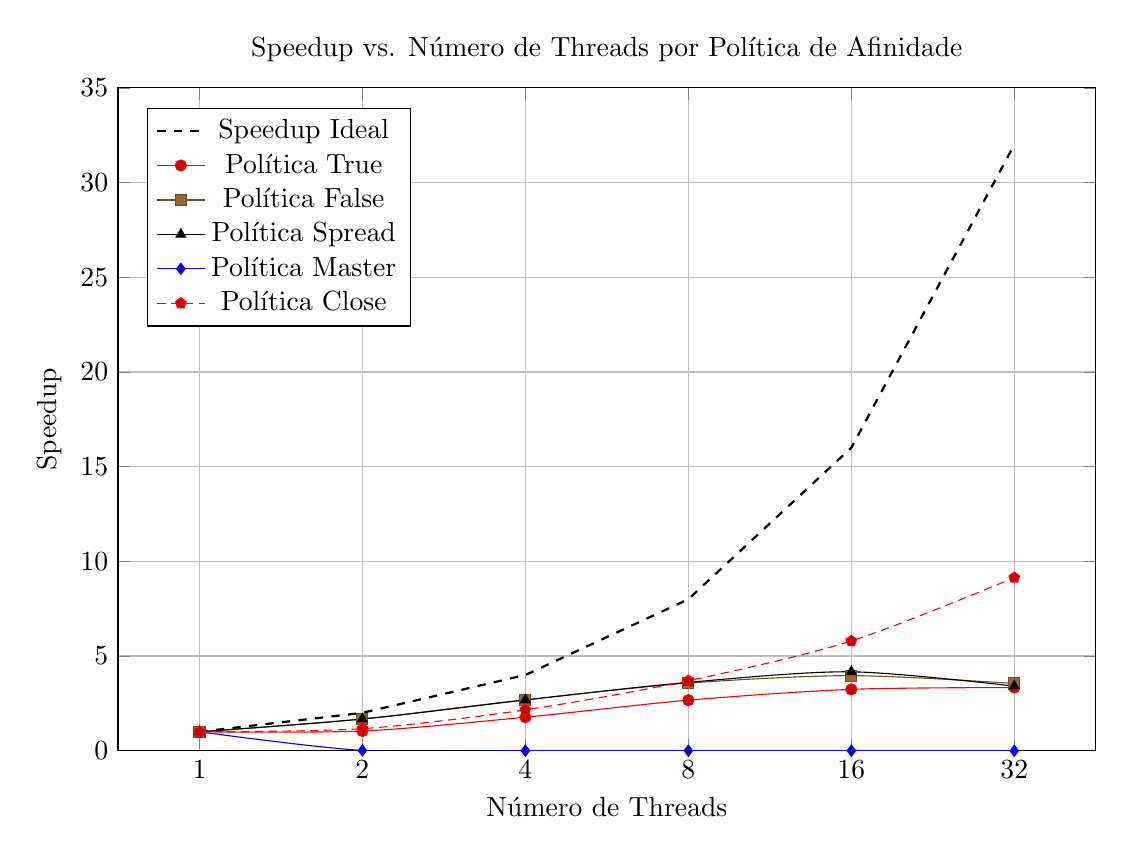
\begin{tikzpicture}
			\begin{axis}[
				title={Speedup vs. Número de Threads por Política de Afinidade},
				xlabel={Número de Threads},
				ylabel={Speedup},
				xmode=log,                      % Eixo X em escala logarítmica
				log ticks with fixed point,     % Formato dos ticks no eixo log
				xtick={1,2,4,8,16,32},
				xticklabels={1,2,4,8,16,32},
				legend pos=north west,          % Posição da legenda
				grid=major,                     % Adiciona grade principal
				width=14cm,                     % Largura do gráfico
				height=10cm,                    % Altura do gráfico
				ymin=0,                         % Valor mínimo do eixo Y
				ymax=35,                        % Ajustado para incluir o speedup ideal de 32
				]
				
				% Curva de Speedup Ideal
				\addplot+[mark=none, dashed, thick, color=black] coordinates {
					(1, 1) (2, 2) (4, 4) (8, 8) (16, 16) (32, 32)
				};
				\addlegendentry{Speedup Ideal}
				
				% Dados para o gráfico - Políticas Reais
				% Politica True
				\addplot+[mark=*, smooth] coordinates {
					(1, 1.000000) (2, 1.041223) (4, 1.770291) (8, 2.670522) (16, 3.241188) (32, 3.337166)
				};
				\addlegendentry{Política True}
				
				% Politica False
				\addplot+[mark=square*, smooth] coordinates {
					(1, 1.000000) (2, 1.681153) (4, 2.691582) (8, 3.568715) (16, 3.965107) (32, 3.553509)
				};
				\addlegendentry{Política False}
				
				% Politica Spread
				\addplot+[mark=triangle*, smooth] coordinates {
					(1, 1.000000) (2, 1.672246) (4, 2.680801) (8, 3.610364) (16, 4.168062) (32, 3.410142)
				};
				\addlegendentry{Política Spread}
				
				% Politica Master
				\addplot+[mark=diamond*, smooth] coordinates {
					(1, 1.000000) (2, 0.014110) (4, 0.004771) (8, 0.002045) (16, 0.000951) (32, 0.000461)
				};
				\addlegendentry{Política Master}
				
				% Politica Close
				\addplot+[mark=pentagon*, smooth] coordinates {
					(1, 1.000000) (2, 1.165592) (4, 2.160008) (8, 3.698040) (16, 5.795370) (32, 9.137857)
				};
				\addlegendentry{Política Close}
				
			\end{axis}
		\end{tikzpicture}
	\end{center}
	
	Para a analise da escalabilidade fraca fixamos o poder computacional no uso de 8 threads e aumentamos o tamanho do problema gradualmente em potencias de 2. Assim podemos verificar qual das políticas melhor se aproximou da eficiência ideal que tem valor igual a 1.
	
	\begin{figure}[h!]
		\centering
		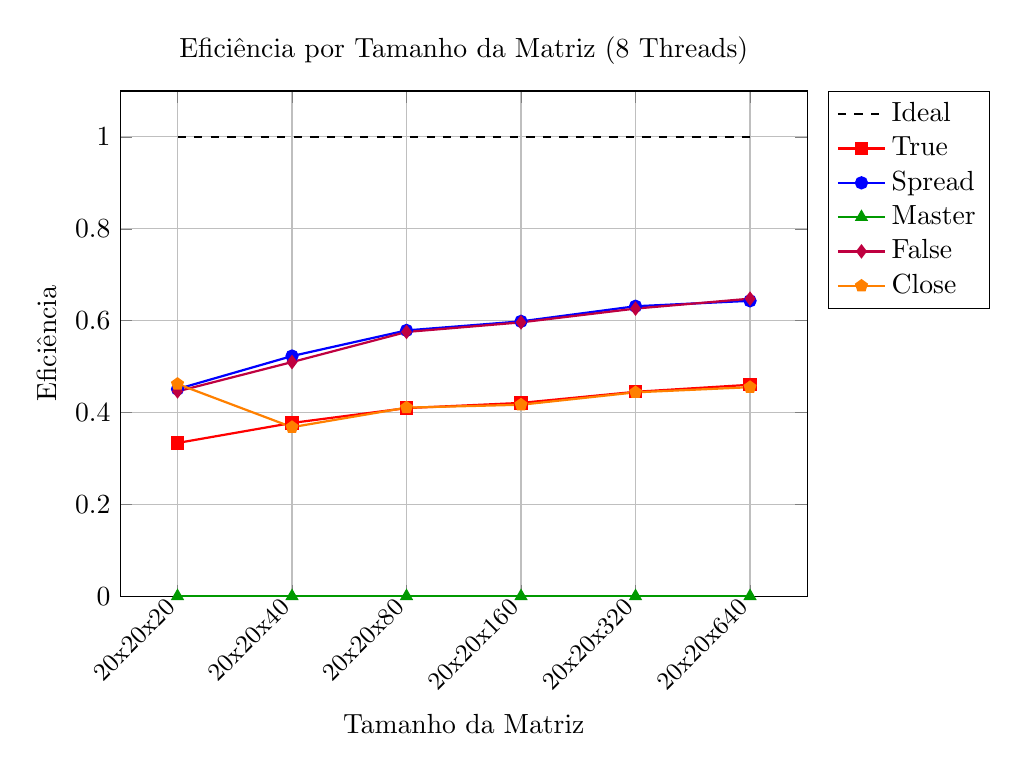
\begin{tikzpicture}
			\begin{axis}[
				title={Eficiência por Tamanho da Matriz (8 Threads)},
				xlabel={Tamanho da Matriz},
				ylabel={Eficiência},
				% Define as coordenadas x como simbólicas para os tamanhos das matrizes
				symbolic x coords={20x20x20, 20x20x40, 20x20x80, 20x20x160, 20x20x320, 20x20x640},
				% Especifica quais ticks mostrar no eixo x
				xtick={20x20x20, 20x20x40, 20x20x80, 20x20x160, 20x20x320, 20x20x640},
				% Rotaciona os rótulos do eixo x para melhor visualização
				x tick label style={rotate=45, anchor=east, font=\small},
				ymin=0,
				ymax=1.1, % Ajustado para melhor visualização da linha de referência e dos dados
				legend pos=outer north east, % Posição da legenda
				legend cell align={left}, % Alinhamento do texto na legenda
				width=0.85\textwidth, % Largura do gráfico relativa à largura do texto
				height=8cm, % Altura do gráfico
				grid=major, % Adiciona grade principal para melhor leitura
				]
				
				% Linha de referência para eficiência = 1 (Ideal)
				\addplot[dashed, black, thick] coordinates {
					(20x20x20, 1) % Ponto inicial da linha de referência
					(20x20x640, 1) % Ponto final da linha de referência
				};
				\addlegendentry{Ideal}

				
				% Dados para a Política "True"
				\addplot[mark=square*, red, thick] coordinates {
					(20x20x20, 0.3338)
					(20x20x40, 0.3774)
					(20x20x80, 0.4097)
					(20x20x160, 0.4210)
					(20x20x320, 0.4452)
					(20x20x640, 0.4605)
				};
				\addlegendentry{True}
				
				% Dados para a Política "Spread"
				\addplot[mark=*, blue, thick] coordinates {
					(20x20x20, 0.4512)
					(20x20x40, 0.5230)
					(20x20x80, 0.5788)
					(20x20x160, 0.5985)
					(20x20x320, 0.6314)
					(20x20x640, 0.6432)
				};
				\addlegendentry{Spread}
				
				% Dados para a Política "Master"
				\addplot[mark=triangle*, green!60!black, thick] coordinates {
					(20x20x20, 0.0003)
					(20x20x40, 0.0003)
					(20x20x80, 0.0003)
					(20x20x160, 0.0003)
					(20x20x320, 0.0002)
					(20x20x640, 0.0003)
				};
				\addlegendentry{Master}
				
				% Dados para a Política "False"
				\addplot[mark=diamond*, purple, thick] coordinates {
					(20x20x20, 0.4461)
					(20x20x40, 0.5099)
					(20x20x80, 0.5754)
					(20x20x160, 0.5963)
					(20x20x320, 0.6263)
					(20x20x640, 0.6479)
				};
				\addlegendentry{False}
				
				% Dados para a Política "Close"
				\addplot[mark=pentagon*, orange, thick] coordinates {
					(20x20x20, 0.4622)
					(20x20x40, 0.3682)
					(20x20x80, 0.4107)
					(20x20x160, 0.4170)
					(20x20x320, 0.4440)
					(20x20x640, 0.4552)
				};
				\addlegendentry{Close}
				
			\end{axis}
		\end{tikzpicture}
		\caption{Comparação da Eficiência de Políticas de Afinidade com 8 Threads}
		\label{fig:eficiencia_politicas_8_threads}
	\end{figure}
		
	\section{Analise dos Resultados}
	
	\hspace{0.62cm}A análise dos resultados obtidos nos permite inferir sobre o comportamento das diferentes políticas de afinidade de threads em dois cenários distintos: escalabilidade forte e escalabilidade fraca.
	
	\subsection{Escala Forte: Speedup vs. Número de Threads}
	\hspace{0.62cm}Observando os gráficos de Speedup em função do número de threads, podemos notar comportamentos bastante distintos entre as políticas:
	
	\begin{itemize}
		\item \textbf{Política Master:} Esta política apresentou o pior desempenho, com um speedup que decai drasticamente com o aumento do número de threads, chegando a valores próximos de zero. Isso indica que forçar todas as threads a executarem no mesmo local da thread principal gerou uma contenção de recursos tão severa que o overhead da paralelização superou qualquer ganho, tornando o programa mais lento do que a versão sequencial em muitos casos. 
		
		\item \textbf{Política True:} A política true demonstrou um speedup modesto, com um crescimento inicial que rapidamente atinge um platô. O speedup máximo parece ser limitado a aproximadamente 3.3x, mesmo com 32 threads. Isso sugere que a política de afinidade herdada ou padrão não está otimizando eficientemente a distribuição das threads para este código, levando a um baixo aproveitamento dos recursos computacionais adicionais.
		
		\item \textbf{Políticas False e Spread:} Ambas as políticas apresentaram um comportamento semelhante, tem o pico de speedup entre 8 e 16 threads e depois observa-se uma queda ao utilizar 32 threads. Isso pode indicar que, com um número muito alto de threads, o custo de comunicação ou a disputa por recursos distribuídos (no caso da spread) ou a migração de threads (no caso da false) começa a superar os benefícios do paralelismo adicional para o tamanho do problema fixado.
		
		\item \textbf{Política Close:} Esta política se destacou por apresentar o melhor speedup com um número maior de threads, chegando a mais de 9x com 32 threads. Isso sugere que agrupar as threads próximas, minimizando a latência de comunicação, foi benéfico para este problema, especialmente quando mais threads são empregadas. O crescimento do speedup parece mais sustentado com o aumento das threads em comparação com false e spread, embora não se aproxime do ideal.
		
	\end{itemize}
	
	\subsection{Escala Fraca: Eficiência vs. Tamanho da Matriz (com 8 Threads)}
	\hspace{0.62cm}Analisando o gráfico de eficiência para a escalabilidade fraca, onde o tamanho do problema por thread é mantido constante (fixando 8 threads e aumentando o tamanho total da matriz):
	
	\begin{itemize}
		\item \textbf{Política Master:} Consistentemente, a política master apresentou uma eficiência próxima de zero para todos os tamanhos de matriz. Isso reforça a conclusão da análise de escala forte: esta política é inadequada para este problema, causando severa degradação de desempenho.
		
		\item \textbf{Políticas Spread e False:} Estas duas políticas foram as que apresentaram a maior eficiência entre as testadas, com valores variando aproximadamente entre 0.45 e 0.65. Ambas demonstram uma tendência de leve aumento da eficiência com o aumento do tamanho da matriz. Isso sugere que, para 8 threads, espalhar as threads (spread) ou deixar o sistema operacional gerenciá-las (false) permite uma utilização razoável dos recursos à medida que o problema cresce. A política false teve uma ligeira vantagem na maioria dos tamanhos de matriz, atingindo a maior eficiência (aproximadamente 0.648).
		
		\item \textbf{Política True:} A política true mostrou uma eficiência moderada, começando em torno de 0.33 e aumentando gradualmente até aproximadamente 0.46. Embora haja uma melhoria com o aumento do tamanho do problema, ela permanece significativamente abaixo das políticas spread e false.
		
		\item \textbf{Política Close:} A política close apresentou um comportamento interessante. Começou com uma eficiência relativamente alta (aproximadamente 0.46 para a menor matriz), similar à true para a maior matriz. No entanto, para o segundo tamanho de matriz (20x20x40), sua eficiência caiu para cerca de 0.37, antes de retomar uma tendência de crescimento gradual com o aumento do problema, alcançando aproximadamente 0.45 para a maior matriz. Essa queda inicial pode indicar que, para problemas menores com 8 threads, agrupar as threads muito próximas pode não ser tão vantajoso, possivelmente devido à sobreposição de caches ou outros recursos locais, antes que o aumento do trabalho por thread compense essa proximidade.
	\end{itemize}
	
	
	\section{Conclusão}

	\hspace{0.62cm}A realização desta tarefa permitiu uma análise aprofundada do impacto das políticas de afinidade de \textit{threads} na escalabilidade de um simulador da equação de Navier-Stokes, evidenciando que a escolha da política exerce influência considerável no desempenho e não é trivial. Os experimentos demonstraram que, enquanto a política \texttt{master} consistentemente degradou o desempenho, as políticas \texttt{false} e \texttt{spread} mostraram-se eficazes para contagens intermediárias de \textit{threads} na escalabilidade forte e foram as mais eficientes na escalabilidade fraca com 8 \textit{threads}. Notavelmente, a política \texttt{close} apresentou o melhor \textit{speedup} com um número elevado de \textit{threads} (32) na escalabilidade forte, sublinhando que a configuração ótima depende das características da aplicação, do volume de dados e do número de \textit{threads}. Nenhuma política atingiu o desempenho ideal, indicando limitações inerentes à paralelização do código ou à arquitetura. Conclui-se que a atividade foi fundamental para consolidar conhecimentos práticos sobre a otimização e avaliação de desempenho em computação paralela, reforçando a necessidade de experimentação para a escolha da política de afinidade mais adequada.
	
	

	 

\end{document}
